\chapter{Morpholigical Processing}

\section{Problem statement}

\begin{enumerate}[(a)]
    \item Implement the morphological operations: erosion, dilation,
    opening and closing, and use the noisy\_fingerprint.tif to check
    your implementation.

    \item Implement boundary extraction, hole filling, connected component extraction.
    Using licoln\_from\_penny.tif, region\_filling\_refletion.tif and chickenfilet\_with\_bones.tif to
    the results, respectively.
\end{enumerate}

\section{Python implementation}

Usage:~\textbf{problem8.py [-h] [--debug] [--test] [--erosion] [--dilation]} \\
\textbf{[--opening] [--closing] [--boundary] [--filling]} \\
\textbf{[--connected]} \\
\textbf{image\_path} \\

Use \textbf{python problem8.py -h} to see the help.

\pagebreak

%\begin{figure}[!htb]\centering
    %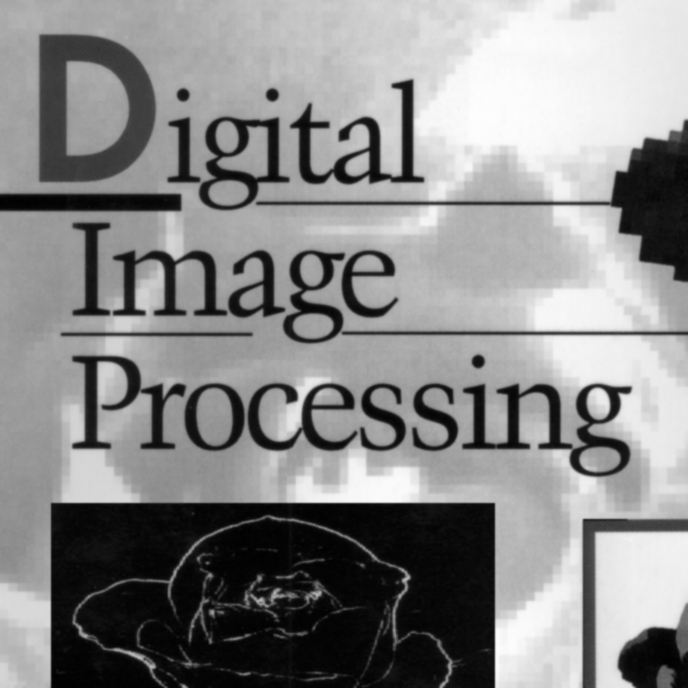
\includegraphics[width=0.6\linewidth]{./images/6/original.jpg}
    %\caption{\small{Original image}}
%\end{figure}

\pagebreak

\section{Erosion}

\textbf{python problem8.py --erosion noisy\_fingerprint.tif}

\begin{figure}[!htb]\centering
    \begin{minipage}{0.45\textwidth}
        \frame{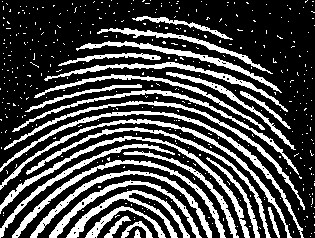
\includegraphics[width=\linewidth]{./images/8/fingerprint.jpg}}
        \caption{\small{Original image}}
    \end{minipage}
    \begin{minipage}{0.45\textwidth}
        \frame{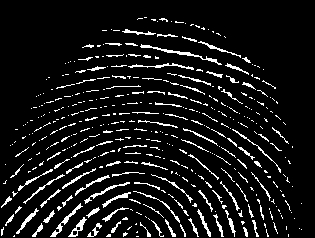
\includegraphics[width=\linewidth]{./images/8/erosion.jpg}}
        \caption{\small{Erosion}}\label{diagram:erosion}
    \end{minipage}
\end{figure}


\section{Dilation}

\textbf{python problem8.py --dilation noisy\_fingerprint.tif}

\begin{figure}[!htb]\centering
    \begin{minipage}{0.45\textwidth}
        \frame{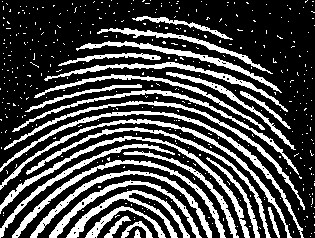
\includegraphics[width=\linewidth]{./images/8/fingerprint.jpg}}
        \caption{\small{Original image}}
    \end{minipage}
    \begin{minipage}{0.45\textwidth}
        \frame{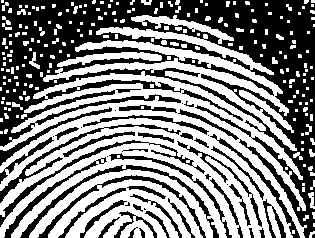
\includegraphics[width=\linewidth]{./images/8/dilation.jpg}}
        \caption{\small{Dilation}}\label{diagram:dilation}
    \end{minipage}
\end{figure}

\pagebreak

\section{Opening}

\textbf{python problem8.py --opening noisy\_fingerprint.tif}

\begin{figure}[!htb]\centering
    \begin{minipage}{0.45\textwidth}
        \frame{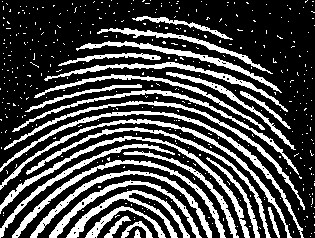
\includegraphics[width=\linewidth]{./images/8/fingerprint.jpg}}
        \caption{\small{Original image}}
    \end{minipage}
    \begin{minipage}{0.45\textwidth}
        \frame{
\includegraphics[width=\linewidth]{./images/8/opening.jpg}}
        \caption{\small{Opening}}\label{diagram:opening}
    \end{minipage}
\end{figure}


\section{Closing}

\textbf{python problem8.py --closing noisy\_fingerprint.tif}

\begin{figure}[!htb]\centering
    \begin{minipage}{0.45\textwidth}
        \frame{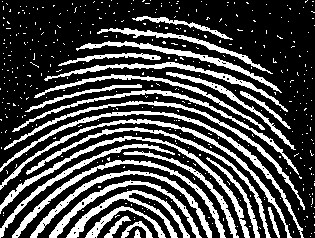
\includegraphics[width=\linewidth]{./images/8/fingerprint.jpg}}
        \caption{\small{Original image}}
    \end{minipage}
    \begin{minipage}{0.45\textwidth}
        \frame{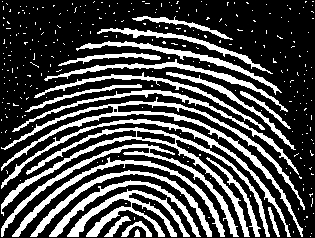
\includegraphics[width=\linewidth]{./images/8/closing.jpg}}
        \caption{\small{Closing}}\label{diagram:closing}
    \end{minipage}
\end{figure}


\pagebreak

\section{Boundary extraction}

\textbf{python problem8.py --boundary licoln\_from\_penny.tif}

\begin{figure}[!htb]\centering
    \begin{minipage}{0.45\textwidth}
        \frame{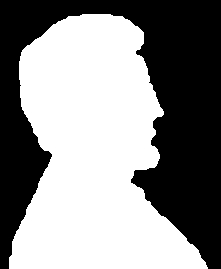
\includegraphics[width=\linewidth]{./images/8/lincoln.jpg}}
        \caption{\small{Original image}}
    \end{minipage}
    \begin{minipage}{0.45\textwidth}
        \frame{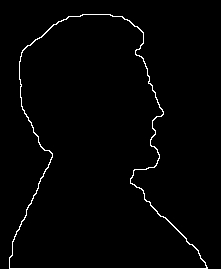
\includegraphics[width=\linewidth]{./images/8/boundary.jpg}}
        \caption{\small{Boundary extraction}}\label{diagram:boundary}
    \end{minipage}
\end{figure}


\section{Hole filling}

\textbf{python problem8.py --filling region\_filling\_reflections.tif}

\begin{figure}[!htb]\centering
    \begin{minipage}{0.45\textwidth}
        \frame{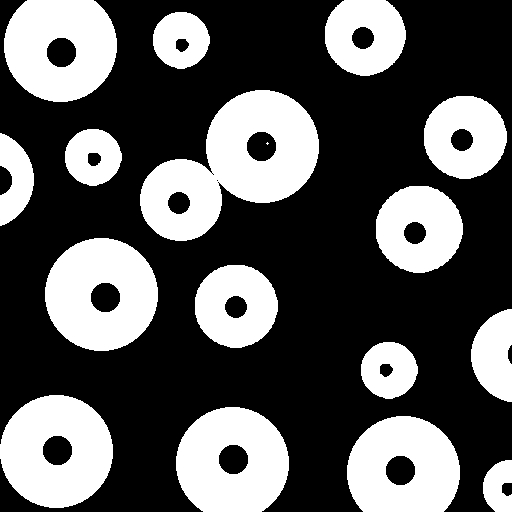
\includegraphics[width=\linewidth]{./images/8/region.jpg}}
        \caption{\small{Original image}}
    \end{minipage}
    \begin{minipage}{0.45\textwidth}
        \frame{
\includegraphics[width=\linewidth]{./images/8/filling.jpg}}
        \caption{\small{Hole filling}}\label{diagram:filling}
    \end{minipage}
\end{figure}

\pagebreak

\section{Connected component extraction}

\textbf{python problem8.py --connected chickenfilet\_with\_bones.tif}

\begin{figure}[!htb]\centering
    \begin{minipage}{0.45\textwidth}
        \frame{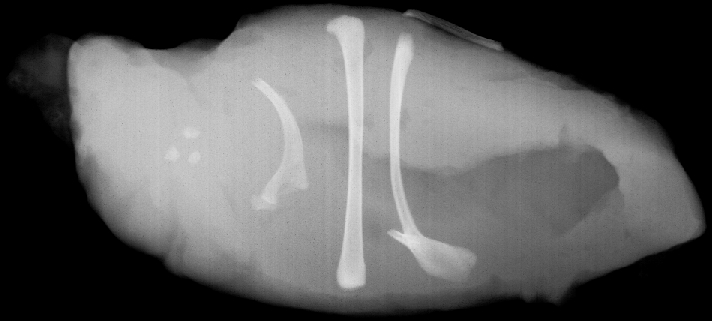
\includegraphics[width=\linewidth]{./images/8/chicken.jpg}}
        \caption{\small{Original image}}
    \end{minipage}
    \begin{minipage}{0.45\textwidth}
        \frame{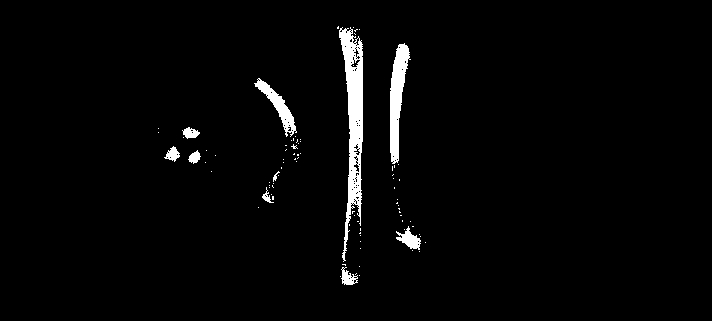
\includegraphics[width=\linewidth]{./images/8/connected_threshold.jpg}}
        \caption{\small{Thresholding}}\label{diagram:connected_threshold}
    \end{minipage}
\end{figure}

\begin{figure}[!htb]\centering
    \begin{minipage}{0.60\textwidth}
        \frame{
\includegraphics[width=\linewidth]{./images/8/connected_erosion.jpg}}
        \caption{\small{Erosion 5$\times$5}}\label{diagram:connected_erosion}
    \end{minipage}
\end{figure}
\bigskip
Connected components:

\begin{center}
\begin{tabular}{c c}
    Connected component & No of pixels \\
    \hline
    01 & 836 \\
    02 & 690 \\
    03 & 44 \\
    04 & 148 \\
    05 & 1 \\
    06 & 18 \\
    07 & 19 \\
    08 & 26 \\
    09 & 2 \\
    10 & 14 \\
    11 & 11 \\
    12 & 13 \\
    13 & 28 \\
    14 & 87 \\
    15 & 18 \\
\end{tabular}
\end{center}
